\begin{frame}{Motivation: quasiperiodicity + interacting electrons}
{
\centering
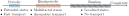
\includegraphics[width=0.5\textwidth]{img/1_motivation/complexity}

}

Cold atoms: \textbf{well-controlled} systems, strong \textbf{interactions}

\begin{columns}
\begin{column}{0.4\textwidth}
\centering
\includegraphics[height=3.5cm]{img/0_cover/free_two_densities_interaction}
\end{column}
\begin{column}{0.6\textwidth}
\textbf{Quasiperiodicity (QP) + strong interactions?}

Naively: delocalisation, fast transport

\textbf{Results}: 
\begin{itemize}
	\item weak QP: delocalisation, fast transport
	\item strong QP: \textbf{many-body localisation}, no transport
\end{itemize}
\end{column}
\end{columns}
\end{frame}
